\documentclass[12pt,a4paper]{article}
\usepackage{lmodern}

\usepackage{placeins}
\usepackage{amssymb,amsmath}
\usepackage{ifxetex,ifluatex}
\usepackage{fixltx2e} % provides \textsubscript
\ifnum 0\ifxetex 1\fi\ifluatex 1\fi=0 % if pdftex
  \usepackage[T1]{fontenc}
  \usepackage[utf8]{inputenc}
\else % if luatex or xelatex
  \ifxetex
    \usepackage{mathspec}
    \usepackage{xltxtra,xunicode}
  \else
    \usepackage{fontspec}
  \fi
  \defaultfontfeatures{Mapping=tex-text,Scale=MatchLowercase}
  \newcommand{\euro}{€}
\fi
% use upquote if available, for straight quotes in verbatim environments
\IfFileExists{upquote.sty}{\usepackage{upquote}}{}
% use microtype if available
\IfFileExists{microtype.sty}{%
\usepackage{microtype}
\UseMicrotypeSet[protrusion]{basicmath} % disable protrusion for tt fonts
}{}
\usepackage[lmargin = 2cm, rmargin = 2cm, tmargin = 2cm, bmargin = 2.5cm]{geometry}


% Figure Placement:
\usepackage{float}
\let\origfigure\figure
\let\endorigfigure\endfigure
\renewenvironment{figure}[1][2] {
    \expandafter\origfigure\expandafter[H]
} {
    \endorigfigure
}

%%%% Jens %%%%
\usepackage{titlesec}
\DeclareMathOperator*{\argmax}{arg\,max}
\DeclareMathOperator*{\argmin}{arg\,min}
\renewcommand{\vec}{\operatorname{vec}}
\newcommand{\tr}{\operatorname{tr}}
\newcommand{\Var}{\operatorname{Var}} % Variance
\newcommand{\VAR}{\operatorname{VAR}} % Vector autoregression
\newcommand{\Lag}{\operatorname{L}} % Lag operator
\newcommand{\Cov}{\operatorname{Cov}}
\newcommand{\diag}{\operatorname{diag}}
\newcommand{\adj}{\operatorname{adj}}
\newcommand{\loglik}{\operatorname{ll}}

\usepackage{centernot}

\allowdisplaybreaks

\titleformat{\section}
{\normalfont\large\bfseries}{\thesection}{1em}{}

\newcommand{\tmpsection}[1]{}
\let\tmpsection=\section
\renewcommand{\section}[1]{\tmpsection{\underline{#1}} }





%% citation setup
\usepackage{csquotes}

\usepackage[backend=biber, maxbibnames = 99, style = apa]{biblatex}
\setlength\bibitemsep{1.5\itemsep}
\addbibresource{R_packages.bib}
\usepackage{color}
\usepackage{fancyvrb}
\newcommand{\VerbBar}{|}
\newcommand{\VERB}{\Verb[commandchars=\\\{\}]}
\DefineVerbatimEnvironment{Highlighting}{Verbatim}{commandchars=\\\{\}}
% Add ',fontsize=\small' for more characters per line
\usepackage{framed}
\definecolor{shadecolor}{RGB}{248,248,248}
\newenvironment{Shaded}{\begin{snugshade}}{\end{snugshade}}
\newcommand{\AlertTok}[1]{\textcolor[rgb]{0.94,0.16,0.16}{#1}}
\newcommand{\AnnotationTok}[1]{\textcolor[rgb]{0.56,0.35,0.01}{\textbf{\textit{#1}}}}
\newcommand{\AttributeTok}[1]{\textcolor[rgb]{0.77,0.63,0.00}{#1}}
\newcommand{\BaseNTok}[1]{\textcolor[rgb]{0.00,0.00,0.81}{#1}}
\newcommand{\BuiltInTok}[1]{#1}
\newcommand{\CharTok}[1]{\textcolor[rgb]{0.31,0.60,0.02}{#1}}
\newcommand{\CommentTok}[1]{\textcolor[rgb]{0.56,0.35,0.01}{\textit{#1}}}
\newcommand{\CommentVarTok}[1]{\textcolor[rgb]{0.56,0.35,0.01}{\textbf{\textit{#1}}}}
\newcommand{\ConstantTok}[1]{\textcolor[rgb]{0.00,0.00,0.00}{#1}}
\newcommand{\ControlFlowTok}[1]{\textcolor[rgb]{0.13,0.29,0.53}{\textbf{#1}}}
\newcommand{\DataTypeTok}[1]{\textcolor[rgb]{0.13,0.29,0.53}{#1}}
\newcommand{\DecValTok}[1]{\textcolor[rgb]{0.00,0.00,0.81}{#1}}
\newcommand{\DocumentationTok}[1]{\textcolor[rgb]{0.56,0.35,0.01}{\textbf{\textit{#1}}}}
\newcommand{\ErrorTok}[1]{\textcolor[rgb]{0.64,0.00,0.00}{\textbf{#1}}}
\newcommand{\ExtensionTok}[1]{#1}
\newcommand{\FloatTok}[1]{\textcolor[rgb]{0.00,0.00,0.81}{#1}}
\newcommand{\FunctionTok}[1]{\textcolor[rgb]{0.00,0.00,0.00}{#1}}
\newcommand{\ImportTok}[1]{#1}
\newcommand{\InformationTok}[1]{\textcolor[rgb]{0.56,0.35,0.01}{\textbf{\textit{#1}}}}
\newcommand{\KeywordTok}[1]{\textcolor[rgb]{0.13,0.29,0.53}{\textbf{#1}}}
\newcommand{\NormalTok}[1]{#1}
\newcommand{\OperatorTok}[1]{\textcolor[rgb]{0.81,0.36,0.00}{\textbf{#1}}}
\newcommand{\OtherTok}[1]{\textcolor[rgb]{0.56,0.35,0.01}{#1}}
\newcommand{\PreprocessorTok}[1]{\textcolor[rgb]{0.56,0.35,0.01}{\textit{#1}}}
\newcommand{\RegionMarkerTok}[1]{#1}
\newcommand{\SpecialCharTok}[1]{\textcolor[rgb]{0.00,0.00,0.00}{#1}}
\newcommand{\SpecialStringTok}[1]{\textcolor[rgb]{0.31,0.60,0.02}{#1}}
\newcommand{\StringTok}[1]{\textcolor[rgb]{0.31,0.60,0.02}{#1}}
\newcommand{\VariableTok}[1]{\textcolor[rgb]{0.00,0.00,0.00}{#1}}
\newcommand{\VerbatimStringTok}[1]{\textcolor[rgb]{0.31,0.60,0.02}{#1}}
\newcommand{\WarningTok}[1]{\textcolor[rgb]{0.56,0.35,0.01}{\textbf{\textit{#1}}}}
\usepackage{graphicx}
\makeatletter
\def\maxwidth{\ifdim\Gin@nat@width>\linewidth\linewidth\else\Gin@nat@width\fi}
\def\maxheight{\ifdim\Gin@nat@height>\textheight\textheight\else\Gin@nat@height\fi}
\makeatother
% Scale images if necessary, so that they will not overflow the page
% margins by default, and it is still possible to overwrite the defaults
% using explicit options in \includegraphics[width, height, ...]{}
\setkeys{Gin}{width=\maxwidth,height=\maxheight,keepaspectratio}
\ifxetex
  \usepackage[setpagesize=false, % page size defined by xetex
              unicode=false, % unicode breaks when used with xetex
              xetex]{hyperref}
\else
  \usepackage[unicode=true, linktocpage = TRUE]{hyperref}
\fi
\hypersetup{breaklinks=true,
            bookmarks=true,
            pdfauthor={Dr.~Yannick Hoga},
            pdftitle={Multivariate Time Series Analysis},
            colorlinks=true,
            citecolor=black,
            urlcolor=black,
            linkcolor=black,
            pdfborder={0 0 0}}
\urlstyle{same}  % don't use monospace font for urls
\setlength{\parindent}{0pt}
\setlength{\parskip}{6pt plus 2pt minus 1pt}
\setlength{\emergencystretch}{3em}  % prevent overfull lines
\setcounter{secnumdepth}{5}

%%% Use protect on footnotes to avoid problems with footnotes in titles
\let\rmarkdownfootnote\footnote%
\def\footnote{\protect\rmarkdownfootnote}

%%% Change title format to be more compact
\usepackage{titling}

% Create subtitle command for use in maketitle
\newcommand{\subtitle}[1]{
  \posttitle{
    \begin{center}\large#1\end{center}
    }
}

\setlength{\droptitle}{-2em}
  \title{Multivariate Time Series Analysis}
  \pretitle{\vspace{\droptitle}\centering\huge}
  \posttitle{\par}
\subtitle{Solution Exercise Sheet 4}
  \author{Dr.~Yannick Hoga}
  \preauthor{\centering\large\emph}
  \postauthor{\par}
  \date{}
  \predate{}\postdate{}


%% linespread settings

\usepackage{setspace}

\onehalfspacing


% Language Setup

\usepackage{ifthen}
\usepackage{iflang}
\usepackage[super]{nth}
\usepackage[ngerman, english]{babel}

%Acronyms
\usepackage[printonlyused, withpage, nohyperlinks]{acronym}
\usepackage{changepage}

% Multicols for the Title page
\usepackage{multicol}


% foot


\begin{document}

\selectlanguage{english}

%%%%%%%%%%%%%% Jens %%%%%
\numberwithin{equation}{section}




\restoregeometry


%%% Header 

\begin{minipage}{0.6\textwidth}
University of Duisburg-Essen\\
Faculty of Business Administration and Economics\\
Chair of Econometrics\\
\end{minipage}

%\begin{minipage}{0.4\textwidth}
	\begin{flushright}
	\vspace{-3cm}
	\includegraphics*[width=5cm]{../Includes/duelogo_en.png}\\
	\vspace{.125cm}
	\end{flushright}
%\end{minipage}
%\vspace{.125cm}
\hspace{-0.005cm}Winter Term 2019/2020

\vspace{0.05cm}

\begin{center}
	\vspace{.25cm}
	Dr.~Yannick Hoga \hspace{.5cm} Thilo Reinschlüssel \\
	\vspace{.25cm}
	\textbf{\Large{Multivariate Time Series Analysis}}\\
	\vspace{.25cm}
	\textbf{\large{Solution Exercise Sheet 4}}\\
	\vspace{.125cm}
\end{center}




% body from markdown

\hypertarget{exercise-1-information-criteria}{%
\section{Exercise 1: Information
Criteria}\label{exercise-1-information-criteria}}

Prove Corollary 4.5 from Slide 4-7.

\emph{Solution:}

From Theorem 4.4:

\begin{align*}
  C(l) = \log \left(\hat{\Sigma_a} (l) \right) + \dfrac{l}{T} \cdot c_T
\end{align*}

\begin{itemize}
  \item[i)] $\lim \limits_{T \rightarrow \infty} c_T \longrightarrow \infty$ 
  \item[ii)] $\lim \limits_{T \rightarrow \infty} \dfrac{c_T}{T} \longrightarrow 0$
\end{itemize}

If i) and ii) hold, \(C(l)\) chooses the optimal/correct model.

\begin{itemize}
  \item AIC: $c_T  = 2K^2$
  \begin{align*}
    \lim \limits_{T \rightarrow \infty} c_T & = 2 \ K^2 \centernot\implies \infty
  \end{align*}
  \begin{itemize}
    \item[$\Rightarrow$] not consistent
  \end{itemize}
  \item BIC: $c_T = \log(T)  \cdot K^2$
    \begin{align*}
    \lim \limits_{T \rightarrow \infty} c_T & = \log(T) K^2   \implies \infty \\
    \lim \limits_{T \rightarrow \infty} \dfrac{c_T}{T} & = \dfrac{\log(T)}{T} K^2 \implies 0 
  \end{align*}
  \begin{itemize}
    \item[$\Rightarrow$] consistent
  \end{itemize}
  \item HQ: $c_T = 2 \ \log(\log(T)) \ K^2$
  \begin{align*}
    \lim \limits_{T \rightarrow \infty} c_T & = 2 \ \log(\log(T)) \ K^2 \implies \infty  \\
    \lim \limits_{T \rightarrow \infty} \dfrac{c_T}{T} & = \dfrac{2 \ \log(\log(T)) \ K^2}{T} \implies 0 
  \end{align*}
  \begin{itemize}
    \item[$\Rightarrow$] consistent
  \end{itemize}
\end{itemize}

\hypertarget{exercise-2-varp-data-application}{%
\section{Exercise 2: VAR(p): Data
application}\label{exercise-2-varp-data-application}}

This exercise is concerned with finding an appropriate \(\VAR(p)\) model
for US macroeconomic data. You can find the dataset
\texttt{us\_macrodata.Rda} attached to this exercise sheet in the Moodle
folder for this tutorial. Please use the \texttt{load} command to import
the dataset from your directory into R. There are 5 variables -- CPI,
Real GDP, the unemployment rate, general private investment and the
debt-to-GDP ratio. All series have been sampled quarterly and were
seasonally adjusted before downloaded from FRED.

\begin{Shaded}
\begin{Highlighting}[]
\CommentTok{# loading data}
\KeywordTok{load}\NormalTok{(}\DataTypeTok{file =}\NormalTok{ here}\OperatorTok{::}\KeywordTok{here}\NormalTok{(}\StringTok{"exercise_MTSA/00_data/us_macrodata.Rda"}\NormalTok{))}
\CommentTok{# loading the MTS package}
\KeywordTok{library}\NormalTok{(MTS)}
\end{Highlighting}
\end{Shaded}

\begin{itemize}
  \item[a.)] Plot all time series and judge which time series seem non-stationary. Proceed to compute growth rates of the non-stationary variables.
\end{itemize}

\emph{Solution:}

\begin{Shaded}
\begin{Highlighting}[]
\NormalTok{macmat <-}\StringTok{ }\KeywordTok{data.matrix}\NormalTok{(us.macro_series)}
\KeywordTok{plot.ts}\NormalTok{(macmat)}
\end{Highlighting}
\end{Shaded}

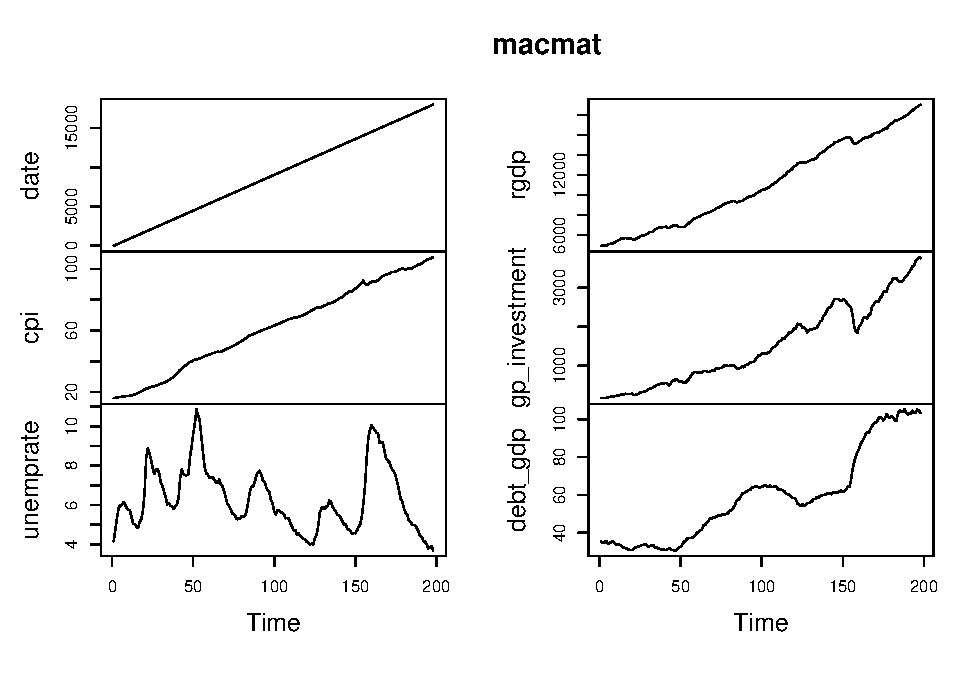
\includegraphics{solution_exercise_5_files/figure-latex/unnamed-chunk-3-1.pdf}

Every series except unemployment looks non-stationary. Regarding the
debt-to-gdp ratio, this is surprising, but we better difference it as
well.

\begin{Shaded}
\begin{Highlighting}[]
\NormalTok{macdata <-}\StringTok{ }\KeywordTok{cbind}\NormalTok{(}\KeywordTok{diff}\NormalTok{(}\KeywordTok{log}\NormalTok{(us.macro_series}\OperatorTok{$}\NormalTok{cpi)), }
\NormalTok{                 us.macro_series}\OperatorTok{$}\NormalTok{unemprate[}\OperatorTok{-}\NormalTok{(}\KeywordTok{nrow}\NormalTok{(macmat))], }
                 \KeywordTok{diff}\NormalTok{(}\KeywordTok{log}\NormalTok{(us.macro_series}\OperatorTok{$}\NormalTok{rgdp)),}
                 \KeywordTok{diff}\NormalTok{(}\KeywordTok{log}\NormalTok{(us.macro_series}\OperatorTok{$}\NormalTok{gp_investment)), }
                 \KeywordTok{diff}\NormalTok{(}\KeywordTok{log}\NormalTok{(us.macro_series}\OperatorTok{$}\NormalTok{debt_gdp)))}

\KeywordTok{plot.ts}\NormalTok{(macdata)}
\end{Highlighting}
\end{Shaded}

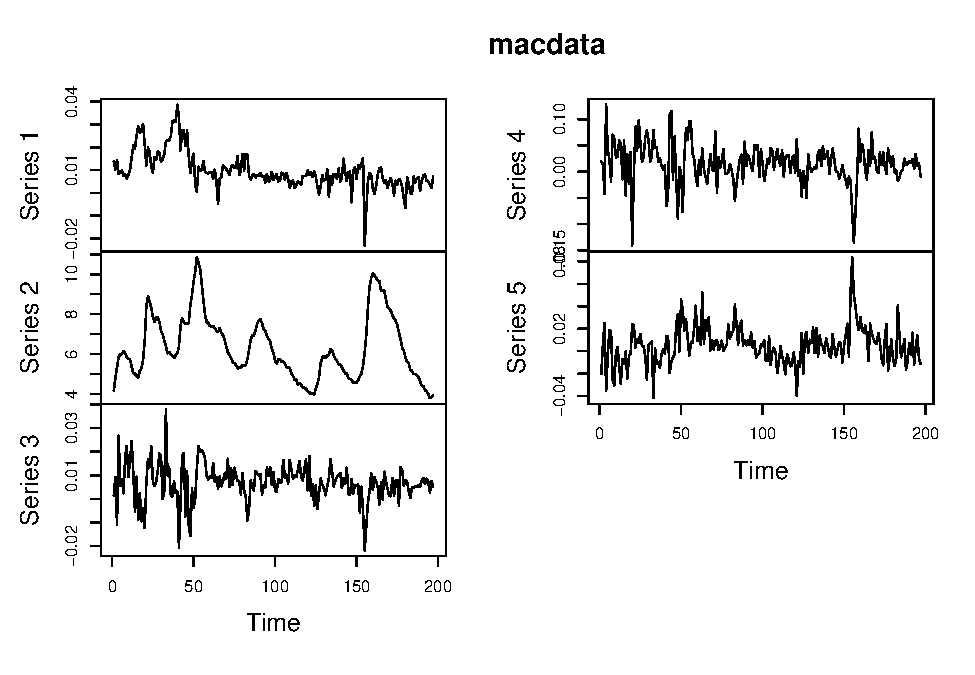
\includegraphics{solution_exercise_5_files/figure-latex/unnamed-chunk-4-1.pdf}

Note that the last observation of \enquote{unemp} was dropped for
conformable length. Its last and not first due to the date information:
measurements are always from the first day of a quarter.

\begin{itemize}
  \item[b.)] Perform a Ljung-Box test on the dataset. Does it look worthwhile to estimate a $\VAR(p)$
\end{itemize}

\emph{Solution:}

\begin{Shaded}
\begin{Highlighting}[]
\KeywordTok{mq}\NormalTok{(}\DataTypeTok{x =}\NormalTok{ macdata, }\DataTypeTok{lag =} \DecValTok{20}\NormalTok{)}
\end{Highlighting}
\end{Shaded}

\begin{verbatim}
## Ljung-Box Statistics:  
##         m       Q(m)     df    p-value
##  [1,]     1       369      25        0
##  [2,]     2       658      50        0
##  [3,]     3       932      75        0
##  [4,]     4      1211     100        0
##  [5,]     5      1430     125        0
##  [6,]     6      1624     150        0
##  [7,]     7      1796     175        0
##  [8,]     8      1953     200        0
##  [9,]     9      2083     225        0
## [10,]    10      2205     250        0
## [11,]    11      2313     275        0
## [12,]    12      2418     300        0
## [13,]    13      2513     325        0
## [14,]    14      2619     350        0
## [15,]    15      2702     375        0
## [16,]    16      2793     400        0
## [17,]    17      2881     425        0
## [18,]    18      2965     450        0
## [19,]    19      3031     475        0
## [20,]    20      3112     500        0
\end{verbatim}

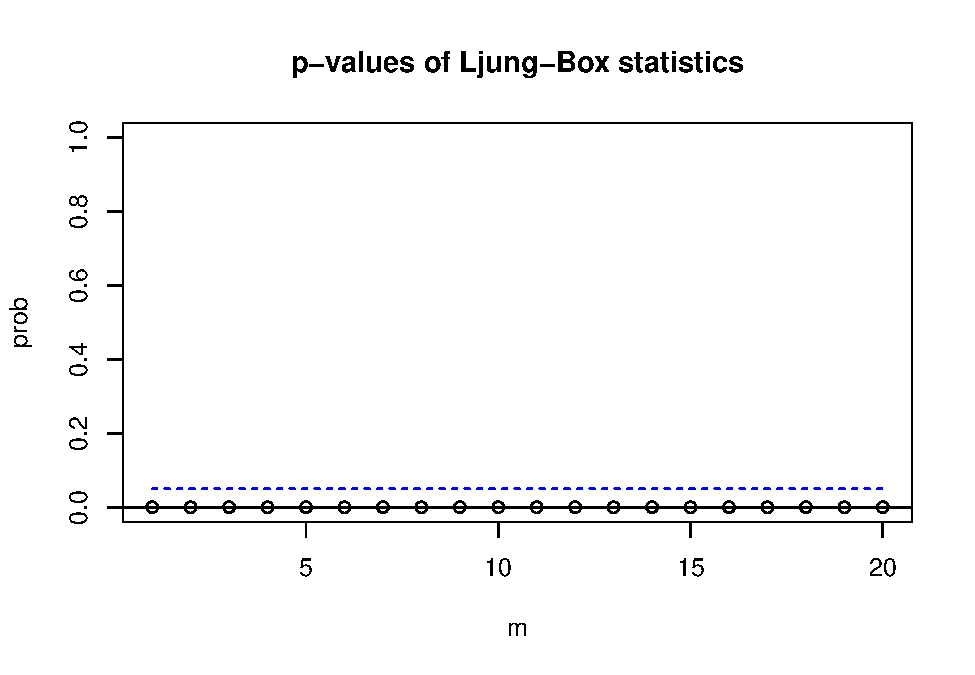
\includegraphics{solution_exercise_5_files/figure-latex/unnamed-chunk-5-1.pdf}

There is some correlation in the dataset.

\begin{Shaded}
\begin{Highlighting}[]
\KeywordTok{mq}\NormalTok{(}\DataTypeTok{x =}\NormalTok{ macdata[,}\OperatorTok{-}\DecValTok{3}\NormalTok{], }\DataTypeTok{lag =} \DecValTok{20}\NormalTok{)}
\end{Highlighting}
\end{Shaded}

\begin{verbatim}
## Ljung-Box Statistics:  
##         m       Q(m)     df    p-value
##  [1,]     1       337      16        0
##  [2,]     2       607      32        0
##  [3,]     3       866      48        0
##  [4,]     4      1121      64        0
##  [5,]     5      1325      80        0
##  [6,]     6      1502      96        0
##  [7,]     7      1650     112        0
##  [8,]     8      1781     128        0
##  [9,]     9      1894     144        0
## [10,]    10      2003     160        0
## [11,]    11      2101     176        0
## [12,]    12      2197     192        0
## [13,]    13      2278     208        0
## [14,]    14      2372     224        0
## [15,]    15      2444     240        0
## [16,]    16      2518     256        0
## [17,]    17      2589     272        0
## [18,]    18      2651     288        0
## [19,]    19      2702     304        0
## [20,]    20      2761     320        0
\end{verbatim}

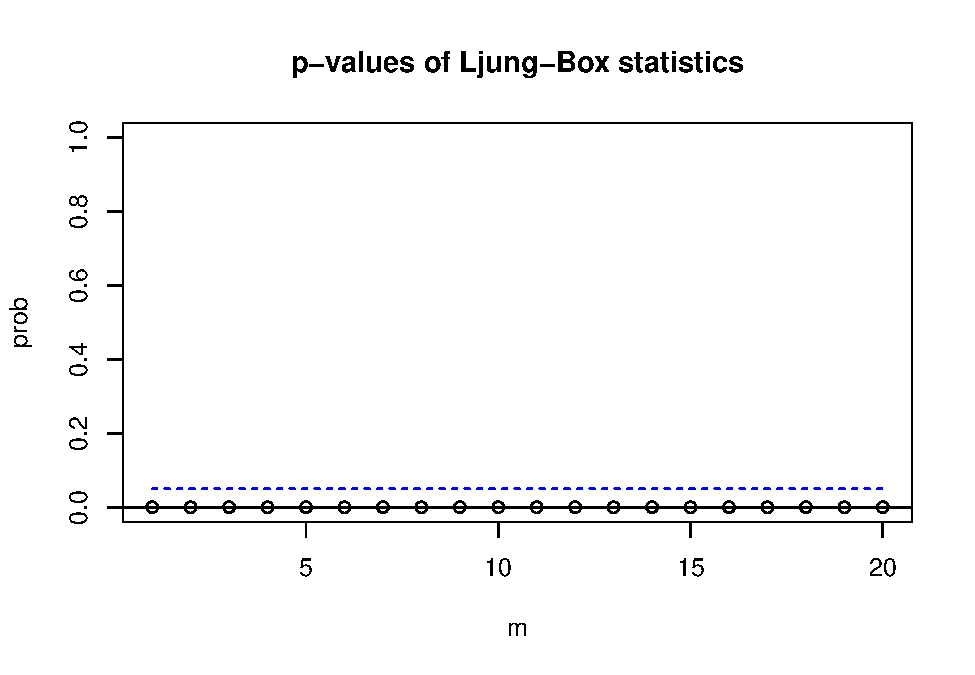
\includegraphics{solution_exercise_5_files/figure-latex/unnamed-chunk-6-1.pdf}

Even without unemployment, there is some correlation in the dataset.

\begin{itemize}
  \item[c.)] Determine the length of the time series. How many coefficients can be estimated and what does it mean for $K$ and $p$?
\end{itemize}

\emph{Solution:}

We have \(T \cdot K\) data points and we estimate \(K^2\) parameters for
each lag. For the intercept we estimate \(K\) parameters. Which leads to
the following condition for the maximal number of lag(s) \(p\):

\[ \dfrac{K \cdot (T -1)}{K^2} \geq p\]

\begin{Shaded}
\begin{Highlighting}[]
\NormalTok{data_dim <-}\StringTok{ }\KeywordTok{dim}\NormalTok{(macdata) }

\NormalTok{Tmax <-}\StringTok{ }\NormalTok{data_dim[}\DecValTok{1}\NormalTok{] }\CommentTok{# observations}
\NormalTok{K <-}\StringTok{ }\NormalTok{data_dim[}\DecValTok{2}\NormalTok{] }\CommentTok{# variables}
\NormalTok{(max.p <-}\StringTok{ }\NormalTok{(Tmax }\OperatorTok{*}\StringTok{ }\NormalTok{K }\OperatorTok{-}\StringTok{ }\NormalTok{K) }\OperatorTok{/}\StringTok{ }\NormalTok{K}\OperatorTok{^}\DecValTok{2}\NormalTok{ )}
\end{Highlighting}
\end{Shaded}

\begin{verbatim}
## [1] 39.2
\end{verbatim}

39 lags can be estimated in addition to the intercept.

\begin{itemize}
  \item[d.)] Consult the AIC, BIC and HQ to determine the optimal lag order for a $\VAR(p)$ model for the whole dataset. Plot the values of the three criteria for the lag orders p from 1 to 5 in one plot.
\end{itemize}

\textbf{Hint: 'VARorder'}

\emph{Solution:}

\begin{Shaded}
\begin{Highlighting}[]
\NormalTok{M <-}\StringTok{ }\DecValTok{10} \CommentTok{# maximal p }
\KeywordTok{VARorder}\NormalTok{(}\DataTypeTok{x =}\NormalTok{ macdata, }\DataTypeTok{maxp =}\NormalTok{ M)}
\end{Highlighting}
\end{Shaded}

\begin{verbatim}
## selected order: aic =  4 
## selected order: bic =  1 
## selected order: hq =  2 
## Summary table:  
##        p      AIC      BIC       HQ     M(p) p-value
##  [1,]  0 -34.8741 -34.8741 -34.8741   0.0000  0.0000
##  [2,]  1 -40.1273 -39.7107 -39.9587 994.0213  0.0000
##  [3,]  2 -40.4982 -39.6649 -40.1608 109.6255  0.0000
##  [4,]  3 -40.6510 -39.4011 -40.1450  69.3340  0.0000
##  [5,]  4 -40.7551 -39.0885 -40.0805  59.2354  0.0001
##  [6,]  5 -40.6962 -38.6129 -39.8529  31.2764  0.1800
##  [7,]  6 -40.5110 -38.0111 -39.4990  10.6681  0.9944
##  [8,]  7 -40.5487 -37.6321 -39.3680  43.8714  0.0112
##  [9,]  8 -40.5490 -37.2158 -39.1997  36.9772  0.0580
## [10,]  9 -40.4934 -36.7436 -38.9754  27.8481  0.3149
## [11,] 10 -40.4553 -36.2888 -38.7687  29.2269  0.2545
\end{verbatim}

\begin{Shaded}
\begin{Highlighting}[]
\CommentTok{# so it's p = 1, 2 or 4.....}
\NormalTok{var1to5.fit <-}\StringTok{ }\KeywordTok{lapply}\NormalTok{(}\DataTypeTok{X =} \DecValTok{1}\OperatorTok{:}\NormalTok{M, }\ControlFlowTok{function}\NormalTok{(i)}
  \KeywordTok{VAR}\NormalTok{(}\DataTypeTok{x =}\NormalTok{ macdata, }\DataTypeTok{include.mean =} \OtherTok{TRUE}\NormalTok{, }\DataTypeTok{p =}\NormalTok{ i, }\DataTypeTok{output =} \OtherTok{FALSE}\NormalTok{))}
\NormalTok{var1to5.aic <-}\StringTok{ }\KeywordTok{sapply}\NormalTok{(}\DecValTok{1}\OperatorTok{:}\NormalTok{M, }\ControlFlowTok{function}\NormalTok{(i) var1to5.fit[[i]]}\OperatorTok{$}\NormalTok{aic)}
\NormalTok{var1to5.bic <-}\StringTok{ }\KeywordTok{sapply}\NormalTok{(}\DecValTok{1}\OperatorTok{:}\NormalTok{M, }\ControlFlowTok{function}\NormalTok{(i) var1to5.fit[[i]]}\OperatorTok{$}\NormalTok{bic)}
\NormalTok{var1to5.hq <-}\StringTok{ }\KeywordTok{sapply}\NormalTok{(}\DecValTok{1}\OperatorTok{:}\NormalTok{M, }\ControlFlowTok{function}\NormalTok{(i) var1to5.fit[[i]]}\OperatorTok{$}\NormalTok{hq)}
\KeywordTok{plot}\NormalTok{(}\DataTypeTok{x =} \DecValTok{1}\OperatorTok{:}\NormalTok{M, }\DataTypeTok{y =}\NormalTok{ var1to5.aic, }\DataTypeTok{type =} \StringTok{"b"}\NormalTok{,}
     \DataTypeTok{main =} \StringTok{"Values of Information Criteria"}\NormalTok{, }\DataTypeTok{xlab =} \StringTok{"p"}\NormalTok{,}
     \DataTypeTok{ylim =} \KeywordTok{c}\NormalTok{( }\KeywordTok{min}\NormalTok{(}\KeywordTok{c}\NormalTok{(var1to5.aic, var1to5.bic, var1to5.hq)), }
               \KeywordTok{max}\NormalTok{(}\KeywordTok{c}\NormalTok{(var1to5.aic, var1to5.bic, var1to5.hq)) ) )}

\KeywordTok{points}\NormalTok{(}\DataTypeTok{x =} \DecValTok{1}\OperatorTok{:}\NormalTok{M, }\DataTypeTok{y =}\NormalTok{ var1to5.bic, }\DataTypeTok{pch =} \DecValTok{11}\NormalTok{, }\DataTypeTok{col =} \StringTok{"red"}\NormalTok{)}
\KeywordTok{points}\NormalTok{(}\DataTypeTok{x =} \DecValTok{1}\OperatorTok{:}\NormalTok{M, }\DataTypeTok{y =}\NormalTok{ var1to5.hq, }\DataTypeTok{col =} \StringTok{"blue"}\NormalTok{, }\DataTypeTok{pch =} \DecValTok{25}\NormalTok{)}
\KeywordTok{legend}\NormalTok{(}\StringTok{"topleft"}\NormalTok{, }\DataTypeTok{legend =} \KeywordTok{c}\NormalTok{(}\StringTok{"AIC"}\NormalTok{, }\StringTok{"BIC"}\NormalTok{, }\StringTok{"HQ"}\NormalTok{), }
       \DataTypeTok{col =} \KeywordTok{c}\NormalTok{(}\StringTok{"black"}\NormalTok{, }\StringTok{"red"}\NormalTok{, }\StringTok{"blue"}\NormalTok{), }
       \DataTypeTok{pch =} \KeywordTok{c}\NormalTok{(}\OtherTok{NA}\NormalTok{, }\DecValTok{11}\NormalTok{, }\DecValTok{25}\NormalTok{), }\DataTypeTok{lwd =} \KeywordTok{c}\NormalTok{(}\DecValTok{2}\NormalTok{, }\OtherTok{NA}\NormalTok{, }\OtherTok{NA}\NormalTok{))}
\end{Highlighting}
\end{Shaded}

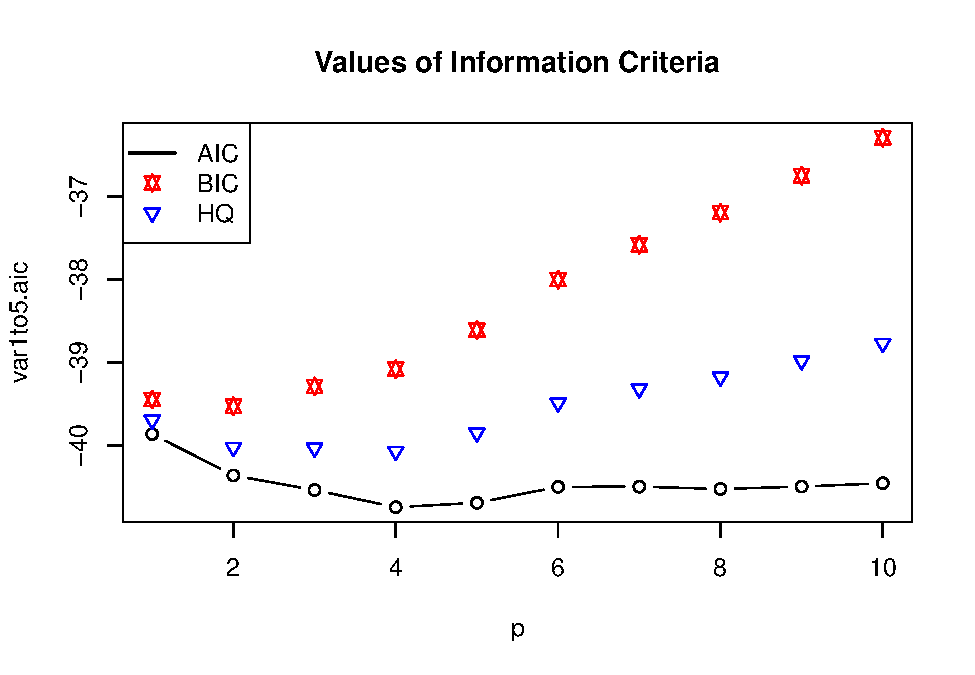
\includegraphics{solution_exercise_5_files/figure-latex/unnamed-chunk-8-1.pdf}

\begin{itemize}
\tightlist
\item
  AIC and HQ are flat around the minima \(\Rightarrow\) no distinct
  optimum visible.
\item
  Conceivable reasons: persistence, omitted variables, wrong functional
  form

  \begin{itemize}
  \tightlist
  \item
    The \(\VAR\) may just work as an approximation
  \end{itemize}
\item
  BIC is the most conservative IC
\item
  Mimima at:
\end{itemize}

\begin{align*}
p = 
  \begin{cases}
  1 & BIC \\
  2 & HQ \\
  4 & AIC
  \end{cases}
\end{align*}

\end{document}
